\subsection{New Designs} %TODO rename title

Five additional designs were generated to compare against the provided designs.
They may be seen in figures \ref{fig:ours_1}, \ref{fig:ours_2}, \ref{fig:ours_3}, \ref{fig:ours_4} and \ref{fig:ours_5}. %Do 1-5 instead? lol
%how was the first design inspired.
Design seven (figure \ref{fig:ours_2}) was an attempt to improve the most efficient design given (design five) by reducing the material used.
Designs eight and ten (figures \ref{fig:ours_3} and \ref{fig:ours_5}) are similar to the designs provided but have different heights.
The efficiency for each design is presented in table \ref{tbl:stiffness2}
 
 \begin{figure*}[p]
    \centering
    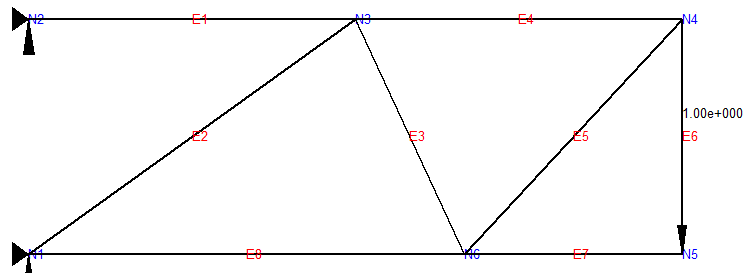
\includegraphics[width=0.6\textwidth]{images/truss1_ours}
    \caption{Design Six}
    \label{fig:ours_1}
\end{figure*}

 \begin{figure*}[p]
    \centering
    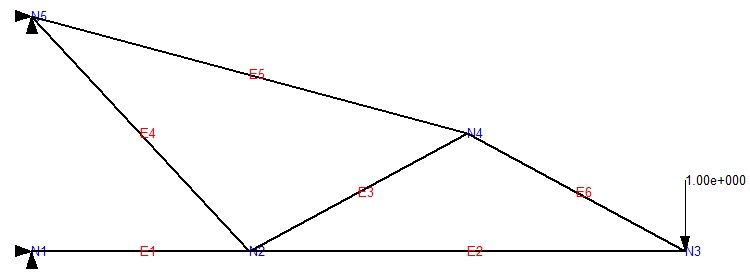
\includegraphics[width=0.6\textwidth]{images/truss2_ours}
    \caption{Design Seven}
    \label{fig:ours_2}
\end{figure*}

 \begin{figure*}[p]
    \centering
    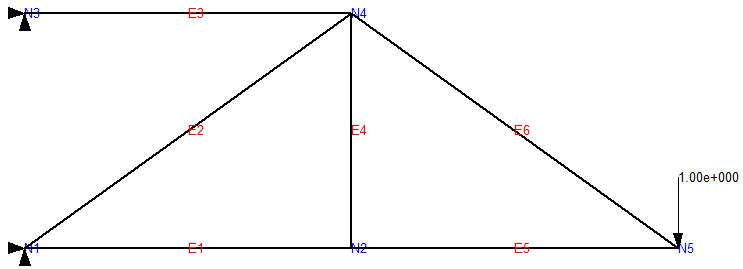
\includegraphics[width=0.6\textwidth]{images/truss3_ours}
    \caption{Design Eight (Height of 10 cm)}
    \label{fig:ours_3}
\end{figure*}

 \begin{figure*}[p]
    \centering
    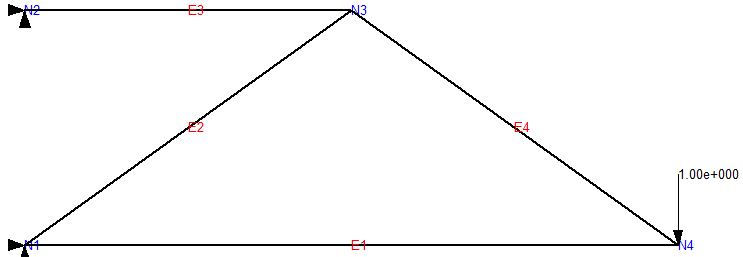
\includegraphics[width=0.6\textwidth]{images/truss4_ours}
    \caption{Design Nine}
    \label{fig:ours_4}
\end{figure*}

 \begin{figure*}[p]
    \centering
    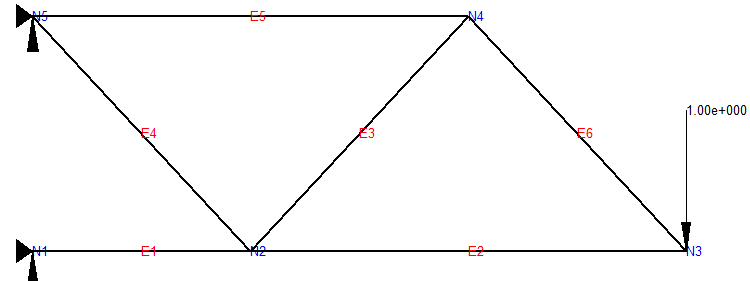
\includegraphics[width=0.6\textwidth]{images/truss5_ours}
    \caption{Design Ten (Height of 5 cm)}
    \label{fig:ours_5}
\end{figure*}


\begin{table*}[hp]
	\centering
	\caption{Stiffness and Efficiency - New Designs (96 GPa)}
	\label{tbl:stiffness2}
	\vspace{6pt}
	\begin{tabular}{lcccccc}
		\toprule
		Design &  \multicolumn{3}{c}{Stiffness} & \multicolumn{3}{c}{Efficiency} \\
		\cmidrule(r){2-4}
		\cmidrule(r){5-7}
		 & Applied Force & Deflection & Stiffness & Material Length & Weight  & Efficiency \\
		\midrule
		6 & 1 N & 0.0133 mm  & 75.2 & 0.991 m & 66.6 g & 1129 \\
		7 & 1 N &  0.0045 mm & 222.7 & 0.871 m & 58.6 g & 3803 \\
		%
		%There has to be something wrong with this:
		8 & 1 N & 0.0017 mm & 602.8 & 0.911 m & 61.2 g & 9848 \\
		%
		9 & 1 N & 0.0042 mm & 237.7 & 0.811 m & 54.5 g &  4364 \\
		10 & 1 N & 0.0122 mm & 82.0 & 0.8354 m & 56.2 g & 1460 \\
		\bottomrule
	\end{tabular}
\end{table*}
